\begin{example}
    Consider a firewall where we initially allow all outgoing packets and block all incoming packets.
    We want to allow incoming packets once a packet is sent outside.
    \begin{center}
        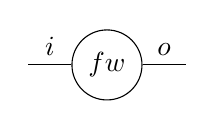
\begin{tikzpicture}[node distance={15mm},main/.style = {draw, circle}]
            \node[main] (s) {$fw$};
            \draw (s) -- node[above]{$i$} (-1,0);
            \draw (s) -- node[above]{$o$} (1,0);
        \end{tikzpicture}
    \end{center}
    We may represent this network with an event structure of
    events $o,i$ for incoming and outgoing packets respectively.
    We assume an empty conflict relation and enabling relation
    $\vdash$ the least one that satisfies:
    \begin{align*}
        \e \vdash i, \e \vdash o
    \end{align*}
    The functions of the causal model are as follows:
    \begin{align*}
        \f{M(\e,i)}    & = Con(\e) = \T                           \\
        \f{M(\e,o)}    & = Con(\e) = \T                           \\
        \f{M(\s{i},o)} & = \F                                     \\
        \f{M(\s{o},i)} & = \F                                     \\
        \f{E(\e,i)}    & = M(\e,i) \wedge Con(\e) = M(\e,i)       \\
        \f{E(\e,o)}    & = M(\e,o) \wedge Con(\e) = M(\e,o)       \\
        \f{E(\s{o},i)} & =
        \left( M(\s{o},i) \vee E(\e,i)  \right) \wedge Con(\s{o}) \\
                       & = M(\s{o},i) \vee E(\e,i)                \\
        \f{E(\s{i},o)} & =
        \left( M(\s{i},o) \vee E(\e,o) \right)
        \wedge Con(\s{i})                                         \\
                       & = M(\s{i},o) \vee E(\e,o)                \\
    \end{align*}
    In the actual context we have:
    \begin{align*}
        \m & \vDash EN(\e,i) = \T    \\
        \m & \vDash EN(\s{o},i) = \T \\
        \m & \vDash EN(\e,o) = \T    \\
        \m & \vDash EN(\s{i},o) = \T \\
        \m & \vDash Con(i,o) = \F    \\
    \end{align*}
    Let $\mathrm{E'} = \mathfrak{E}(\vec V) = (\s{i,o},\e,\vdash')$ 
    in the actual context where we have:
    \begin{align*}
        \e \vdash' o, \s{i} \vdash' o, \e \vdash' i, 
        \s{o} \vdash' i
    \end{align*}
    Now let $\sigma = \s{o}$ be a counterexample.     
    Assume that we want to declare $M(\e,o) = \T$ as a cause of 
    $\sigma \in \mathcal{F}(\mathrm{E'})$ using $(\e,\e,\F)$ as a witness.
    It is easy to verify that $\mathrm{E'}$ is an event structure.
    To check whether $\sigma$ is a configuration of $\mathrm{E'}$ we need
    to have $\e \vdash' o$ which is satisfied.
    Thus we have:
    \begin{align*}
        \m \vDash M(\e,o) = \T \wedge \sigma 
        \in \mathcal{F}(\mathfrak{E}(\vec V)) \wedge \vec v \in \mathcal{E}
    \end{align*}
    Thus, the AC1 condition is satisfied.
    Next, we need to verify the AC2 conditions.
    Assume that we set $M(\e,o)$ to false.
    $E(\e,o)$ depends on $M(\e,o)$ and $E(\s{o},i)$ depends on $E(\e,o)$,
    and these are the only variables that are affected by changing $M(\e,o)$.
    Thus, we have:
    \begin{align*}
        \m & \vDash [M(\e,o)\la \F] EN(\e,i) = \T \\
        \m & \vDash [M(\e,o)\la \F] EN(\s{o},i) = \T \\
        \m & \vDash [M(\e,o)\la \F] EN(\e,o) = \F \\
        \m & \vDash [M(\e,o)\la \F] EN(\s{i},o) = \F 
    \end{align*}
    Let $\vec v'$ be the value of endogenous variables after setting 
    $M(\e,o)$ to false so we have $\m \vDash [M(\e,o)\la \F]\vec V = \vec v'$.
    Let $\mathrm{E}'' = \mathfrak{E}(\vec V) = (\s{i,o},\e, \vdash'')$ where:
    \begin{align*}
        \e \vdash'' i, \s{o} \vdash'' i
    \end{align*}
    Again we can easily verify that $\mathrm{E}''$ is an event structure.
    Now, since $\e \not \vdash'' o$, thus $\sigma$ is not a configuration of
    the $\mathrm{E}''$, so we have:
    \begin{align*}
        \m \vDash [M(\e,o) \la \F] \sigma \not \in \mathcal{F}(\mathfrak{E}(\vec V))
        \wedge \vec v' \in \mathcal{E}
    \end{align*}
    Which satisfies the AC2(a) condition.
    Since we have used an empty $\vec W$ set for the witness, and AC2(a)
    condition is satisfied, thus we can conclude that $M(\e,o) = \T$ is a 
    cause of $\sigma \in \mathcal{F}(\mathrm{\mathfrak{E}(\vec V)})$.
\end{example}

\begin{example}
    Consider the following network where we have
    a stateful firewall on the switch $s$.
    Initially, we allow outgoing packets from $a$ and
    block all incoming packets from either $b$ or $c$.
    Assume that packets from $a$ are broadcasted to
    both $b$ and $c$ and we wish to allow traffic
    from both of them afterward.
    \begin{center}
        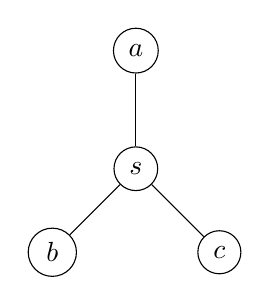
\begin{tikzpicture}[node distance={15mm},main/.style = {draw, circle}]
            \node[main] (s) {$s$};
            \node[main] (a) [above of=s] {$a$};
            \node[main] (b) [below left of=s] {$b$};
            \node[main] (c) [below right of=s] {$c$};
            \draw (s) -- (a);
            \draw (s) -- (b);
            \draw (s) -- (c);
        \end{tikzpicture}
    \end{center}
    We define an event structure where
    $\mathcal{E} = \s{a,b,c,i}$.
    We let $a,b,c$ to represent the events of sending
    a packet from $a$,$b$ and $c$ to $s$ respectively.
    Let $i$ indicate the event of the forwarding of
    an arbitrary packet from $s$ to $a$ (this may coming
    from either $b$ or $c$).
    We consider an empty conflict relation and enabling
    relation the least one for which we have:
    \begin{align*}
        \e \vdash a,\e \vdash b, \e \vdash c,
        \s{b} \vdash i, \s{c} \vdash i
    \end{align*}
    We may consider the configuration $\sigma = \s{b,c,i}$ as a
    counterexample since $i$ is happened while $a$ has not been happened yet.
    Regarding this event structure we have:
    \begin{align*}
        \f{M(\e,a)}      & = Con(\e) =  \T                                  \\
        \f{M(\e,b)}      & = Con(\e) =  \T                                  \\
        \f{M(\e,c)}      & = Con(\e) = \T                                   \\
        \f{M(\s{b},i)}   & = Con(\s{b}) =  \T                               \\
        \f{M(\s{c},i)}   & = Con(\s{c}) =  \T                               \\
        \f{E(\e,b)}      & = M(\e,b) \wedge Con(\e) = M(\e,b)               \\
        \f{E(\s{b},c)}   & = (M(\s{b},c) \vee E(\e,c)) \wedge Con(\s{b})    \\
                         & = M(\s{b},c) \vee E(\e,c)                        \\
        \f{E(\e,c)}      & = M(\e,c) \wedge Con(\e)  = M(\e,c)              \\
        \f{E(\s{b,c},i)} & = (M(\s{b,c},i) \vee E(\s{b},i) \vee E(\s{c},i))
        \wedge Con(\s{b,c})                                                 \\
        \f{E(\s{b},i)}   & = (M(\s{b},i) \vee E(\e,i))\wedge Con(\s{b})     \\
                         & = M(\s{b},i) \vee E(\e,i)                        \\
        \f{E(\s{c},i)}   & = (M(\s{c},i) \vee E(\e,i))\wedge Con(\s{c})     \\
                         & = M(\s{c},i) \vee E(\e,i)                        \\
    \end{align*}
    Let $\pi = b,c,i$ be a permutation of $\sigma$, we have:
    \begin{align*}
        \varphi_{\pi} & =
        E(\e,b) \wedge E(\s{b},c) \wedge E(\s{b,c},i)
        \wedge Con(\sigma)                            \\
        \varphi       & = \varphi_{\pi} \vee \varphi'
    \end{align*}
    Here we can declare $M(\s{b},i) = \T$ as a cause of $\varphi$.
    Let $(M(\s{c},i),\F,\F)$ be the witness.
    We need to verify the following conditions:
    \begin{itemize}
        \item AC1:  $\m \vDash M(\s{b},i) = \T \wedge \varphi$
        \item AC2(a): $\m\vDash [M(\s{b},i)\la \F,M(\s{c},i)\leftarrow \F] \neg \varphi$
        \item AC2(b): $\m \vDash [\vec W' \la \vec w', \vec Z' \la \vec z^* ]\varphi$
              for all subsets
              $\vec W'$ of $\vec W$ and $\vec Z'$ of $\vec Z$.
    \end{itemize}
    First, observe that since $M(\e,b)$ is true thus $E(\e,b)$ is true.
    Also, since $M(\e,c)$ is true, so $E(\s{b},c)$ is true too.
    Finally, $M(\s{b},i)$ and subsequently $E(\s{b},i)$ is true which makes
    $E(\s{b,c},i)$ true.
    So we can conclude that $\varphi$ is true in the actual context and
    AC1 is satisfied.

    For verifying the AC2(a) condition notice that setting both of
    $M(\s{b},i)$ and $M(\s{c},i)$ to false results in
    $E(\s{b},i)$ and $E(\s{c},i)$ become false.
    Now, since $M(\s{b,c},i)$ is false too, all three terms of the first
    conjunction of $\f{E(\s{b,c},i)}$ are false so $E(\s{b,c},i)$ becomes false.
    We can finally conclude that $\varphi$ becomes false too.
    To verify the AC2(b) condition, first we need to set $M(\s{c},i)$ to false.
    This setting has no effect on $E(\e,b)$, $E(\s{b},c)$ and $E(\s{b},i)$.
    Also note that $E(\s{b},i)$ is true in the actual context and it is
    not affected by $M(\s{c},i)$, so it remains true by setting
    any $\vec Z'$ to $\vec z^*$.
    Thus, the disjunction of $E(\s{b,c},i)$ has a true value and thus it
    remains true even if we set $E(\s{c},i)$ to false.
    We can conclude that $\varphi$ remains true and AC2(b) is satisfied.
\end{example}

\begin{example}
    Consider the following network where wish to forward traffic from $a$ to $b$ and $x$ to $y$.
    But, we also want to limit the traffic on the link 3 so that at any moment
    there must be at most one packet traversing this link.
    \begin{center}
        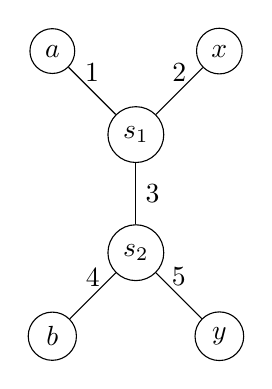
\begin{tikzpicture}[node distance={15mm},main/.style = {draw, circle}]
            \node[main] (s1) {$s_1$};
            \node[main] (s2) [below of=s1] {$s_2$};
            \node[main] (a) [above left of=s1]{$a$};
            \node[main] (x) [above right of=s1]{$x$};
            \node[main] (b) [below left of=s2]{$b$};
            \node[main] (y) [below right of=s2]{$y$};
            \draw (a) --  node[above]{1} (s1);
            \draw (x) --  node[above]{2}(s1);
            \draw (s1) --  node[right]{3}(s2);
            \draw (b) --  node[above]{4}(s2);
            \draw (y) --  node[above]{5}(s2);
        \end{tikzpicture}
    \end{center}
    We define events $a,x,b,y$ representing the forwarding of a packet from
    1 to 3, 2 to 3, 3 to 4, and 3 to 5 respectively.
    We define an event $c$ when congestion is detected on link 3 (at least two packets are being traversed through the link).
    We define the conflict relation in such a way that we have:
    \begin{align*}
        a \# y, x\# b
    \end{align*}
    We consider an enabling relation the least one for which we have:
    \begin{align*}
        \e \vdash a, \e \vdash x, \s{a} \vdash b, \s{x} \vdash y,
        \s{a,x} \vdash c
    \end{align*}
    Now, consider $\sigma = \s{a,x,c}$ as a counterexample.
    The functions of the causal model are as follows:
    \begin{align*}
        \f{M(\e,a)}      & = Con(\e) = \T                     \\
        \f{M(\e,x)}      & = Con(\e) = \T                     \\
        \f{M(\s{a},b)}   & = Con(\s{a}) = \T                  \\
        \f{M(\s{x},y)}   & = Con(\s{x}) = \T                  \\
        \f{M(\s{a,x},c)} & = Con(\s{a,x})                     \\
        \varphi_{\pi}    & = E(\e,a) \wedge E(\s{a},x) \wedge
        E(\s{a,x},c) \wedge Con(\s{a,x,c})                    \\
        \f{E(\e,a)}      & = M(\e,a) \wedge Con(\e) = M(\e,a) \\
        \f{E(\s{a},x)}   & = (M(\s{a},x) \vee E(\e,x) )
        \wedge Con(\s{a})                                     \\
        \f{E(\e,x)}      & = M(\e,x) \wedge Con(\e) = M(\e,x) \\
        \f{E(\s{a,x},c)} & = (M(\s{a,x},c) \vee E(\s{a},c)
        \vee E(\s{x},c)) \wedge Con(\s{a,x})                  \\
        \f{E(\s{a},c)}   & = (M(\s{a},c) \vee E(\e,c))
        \wedge Con(\s{a})                                     \\
                         & = M(\s{a},c) \vee E(\e,c)          \\
        \f{E(\s{x},c)}   & = (M(\s{x},c) \vee E(\e,c))
        \wedge Con(\s{x})                                     \\
                         & = M(\s{x},c) \vee E(\e,c)          \\
    \end{align*}
    In this example, we may introduce $M(\e,x) = \T$ as a cause of $\varphi$.
    Assume that we set $M(\e,x)$ to false.
    This causes $E(\e,x)$ to become false which cause $E(\s{a},x)$ become false.
    Finally, $E(\s{a},x)$ becoming false causes $\varphi$ to become false.
    Since we have used an empty $\vec W$, and the AC2(a) condition is
    satisfied, so $M(\e,x) = \T$ is a but-for cause of $\varphi$.
\end{example}
